%% Symbolically executing real-world software is challenging not only because of path explosion but also because real-world systems interact with their environment in varied and complex ways. This section describes our experience building \cnine's symbolic model of a POSIX environment, which supports most essential interfaces: threads, process management, sockets, pipes, polling, etc. We believe the described techniques are general enough to model other OSes and environments as well.

In this chapter, we introduce the design principles of a symbolic model for operating system abstractions.  We then present how these principles are used in the \cnine symbolic execution platform for obtaining a symbolic model of a POSIX environment, which supports most essential interfaces: threads, process management, sockets, pipes, polling, etc.

%%%%%%%%%%%%%%%%%%%%%%%%%%%%%%%%%%%%%%%%%%%%%%%%%%%%%%%%%%%%%%%%%%%%%%%%%%%%%%%%

\section{Environment Model Design}

\topic{The goal of a symbolic model is to simulate the behavior of a real execution environment, while maintaining the necessary symbolic state behind the environment interface.}  The symbolic execution engine (SEE) can then seamlessly transition back and forth between the program and the environment.

\topic{While writing and maintaining a model can be laborious and prone to error~\cite{s2eSystem}, there exist cases in
  which models provide distinct advantages.} First, symbolic execution with a model can be substantially faster than without.  For instance, in the Linux kernel, transferring a packet between two hosts exercises the entire TCP/IP networking stack and the associated driver code, amounting to over 30 \kloc.  In contrast, \cnine's POSIX model achieves the same functionality in about 1.5 \kloc. Requirements that complicate a real environment/OS implementation, such as performance and extensibility, can be ignored in a symbolic model. Second, when an interface is as stable as POSIX, investing the time to model it becomes worthwhile.

\topic{We designed a minimal yet general ``symbolic system call'' interface to the \cnine SEE, which provides the essential building blocks for thread context switching, address space isolation, memory sharing, and sleep operations.}  These are hard to provide solely through an external model. We give more details about symbolic system calls in Section~\ref{sec:symbolic-engine-modifications}.

\topic{In some cases, it is practical to have the host OS handle parts of the environment via \emph{external calls}}.  These are implemented by concretizing the symbolic parameters of a system call before invoking it from symbolically executing code. Unlike \cite{dart,klee,exe}, \cnine allows external calls \emph{only} for stateless or read-only system calls, such as reading a system configuration file from the \codebit{/etc} directory.  This restriction ensures that external concrete calls do not clobber other symbolically executing paths.

\begin{figure}[h!]
  \centering
  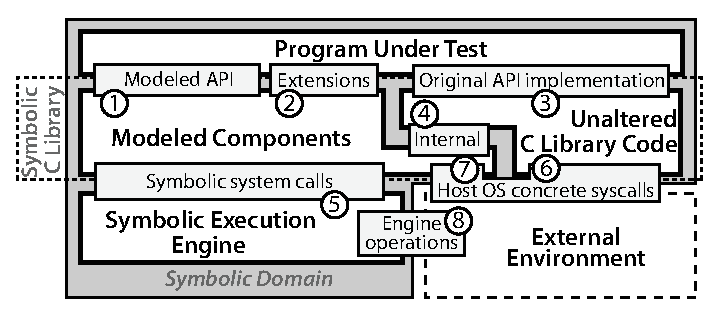
\epsfig{file=figures/cloud9/posix-model.eps, width=3.4in}
  \caption{Architecture of the \cnine POSIX model.}
  \label{fig:posixmodel}
\end{figure}

\cnine builds upon the \klee symbolic execution engine, and so it inherits from \klee the mechanism for replacing parts of the C Library with model code; it also inherits the external calls mechanism.  \cnine adds the symbolic system call interface and replaces parts of the C Library with the POSIX model.  The resulting architecture is shown in Fig.~\ref{fig:posixmodel}.

\newcommand{\cI}{\!{\raisebox{-0.2ex}{\large\ding{192}}}\xspace}
\newcommand{\cII}{\!{\raisebox{-0.2ex}{\large\ding{193}}}\xspace}
\newcommand{\cIII}{\!{\raisebox{-0.2ex}{\large\ding{194}}}\xspace}
\newcommand{\cIV}{\!{\raisebox{-0.2ex}{\large\ding{195}}}\xspace}
\newcommand{\cV}{\!{\raisebox{-0.2ex}{\large\ding{196}}}\xspace}
\newcommand{\cVI}{\!{\raisebox{-0.2ex}{\large\ding{197}}}\xspace}
\newcommand{\cVII}{\!{\raisebox{-0.2ex}{\large\ding{198}}}\xspace}
\newcommand{\cVIII}{\!{\raisebox{-0.2ex}{\large\ding{199}}}\xspace}

\topic{Before symbolic execution starts, the \cnine system links the program under test with a special symbolic C Library.} We built this library by replacing parts of the existing uClibc library in \klee with the POSIX model code.  Developers do not need to modify the code of to-be-tested programs in any way to make it run on \cnine.  

\topic{In the C Library, we replaced operations related to threads, processes, file descriptors, and network operations with their corresponding model \cI, and augmented the API with \cnine-specific extensions \cII.}  A large portion of the C Library is reused, since it works out of the box \cIII (e.g. memory and string operations).  Finally, parts of the original C Library itself use  the modeled code \cIV (e.g., Standard I/O \codebit{stdio} relies on the modeled POSIX file descriptors).

\topic{The modeled POSIX components interface with the SEE through symbolic system calls \cV, listed in Table~\ref{table:primitives}.}  Occasionally, the unmodified part of the C Library invokes external system calls \cVI, and the model code itself needs support from the host OS \cVII---in order to make sure the external calls do not interfere with the symbolic engine's own operations~\cVIII, such access is limited to read-only and/or stateless operations.  This avoids problems like, for instance, allowing an external \codebit{close()} system call to close a network connection or log file that is actually used by the SEE itself.

\begin{table}[!t]
\renewcommand{\arraystretch}{1.1}
\addtolength{\tabcolsep}{-2pt}
{\small
\centering
\begin{tabular}{|l|l|}
\hline
~~~~~\textbf{Primitive Name} & ~~~~~~~~~~~~~~~~\textbf{Description} \\
\hline
 \cninesuffix\_make\_shared & Share object across a CoW domain \\
\hline
\hline
  \cninesuffix\_thread\_create & \multirow{2}{4cm}{Create and destroy threads}\\
  \cninesuffix\_thread\_terminate & \\
  \cline{1-2}
   \cninesuffix\_process\_fork & \multirow{2}{4cm}{Fork and terminate the current process}\\
  \cninesuffix\_process\_terminate & \\
  \cline{1-2}
   \cninesuffix\_get\_context & Get the current context (pid and tid) \\
\hline
\hline
 \cninesuffix\_thread\_preempt & Preempt a thread  \\
 \hline 
 \cninesuffix\_thread\_sleep & Thread sleep on waiting queue \\
 \hline
 \cninesuffix\_thread\_notify & Wake threads from waiting queue \\
 \hline
 \cninesuffix\_get\_wlist & Create a new waiting queue \\
\hline
\end{tabular}
\caption{\cnine  primitives used to build the POSIX model.}
\label{table:primitives}
}
\vspace{-3mm}
\end{table}

%%%%%%%%%%%%%%%%%%%%%%%%%%%%%%%%%%%%%%%%%%%%%%%%%%%%%%%%%%%%%%%%%%%%%%%%%%%%%%%%

\section{Symbolic Execution Engine Primitives}
\label{sec:symbolic-engine-modifications}

\topic{In order to support the POSIX interface, we augmented \klee with two major features:} multiple address spaces per state and support for scheduling threads and processes.  This functionality is accessed by model code through the symbolic system call interface (Table~\ref{table:primitives}).  Additional models of non-POSIX environments can be built using this interface.

\paragraph{Address Spaces}  \topic{\klee uses copy-on-write (CoW) to enable memory sharing between symbolic states.}  We extend this functionality in two ways.  First, we enable multiple address spaces within a single execution state, corresponding to multiple processes encompassed in that state. Address spaces can thus be duplicated both across states (as in classic \klee) and within a state, when \codebit{\cninesuffix\_process\_fork} is invoked, e.g., as used by the POSIX model's \codebit{fork()}.

\topic{Second, we organize the address spaces in an execution state as \emph{CoW domains} that permit memory sharing between processes.}  A memory object can be marked as shared by calling \codebit{\cninesuffix\_\allowbreak{}make\_\allowbreak{}shared}; it is then automatically mapped in the address spaces of the other processes within the CoW domain.  Whenever a shared object is modified in one address space, the new version is automatically propagated to the other members of the CoW domain.  The shared memory objects can then be used by the model as global memory for inter-process communication.

\paragraph{Multithreading and Scheduling}  Threads are created in the currently executing process by calling \codebit{\cninesuffix\_\allowbreak{}thread\_\allowbreak{}create}.  \cnine's POSIX threads (pthreads) model makes use of this primitive in its own \codebit{pthread\_create()} routine.

\topic{\cnine implements a cooperative scheduler:}  An enabled thread runs uninterrupted (atomically), until either (a) the thread goes to sleep; (b) the thread is explicitly preempted by a \codebit{\cninesuffix\_\allowbreak{}thread\_\allowbreak{}preempt} call; or (c) the thread is terminated via symbolic system calls for process/thread termination. Preemption occurs at explicit points in the model code, but it is straightforward to extend \cnine to automatically insert preemptions calls at instruction level (as would be necessary, for instance, when testing for race conditions).

\topic{When \codebit{\cninesuffix\_\allowbreak{}thread\_sleep} is called, the SEE places the current thread on a specified waiting queue, and an enabled thread is selected for execution.}  Another thread may call \codebit{\cninesuffix\_thread\_\allowbreak{}notify} on the waiting queue and wake up one or all of the queued threads.

\topic{\cnine can be configured to schedule the next thread deterministically, or to fork the execution state for each possible next thread.} The latter case is useful when looking for concurrency bugs, but it can be a significant source of path explosion, so it should be disabled when not needed.

\topic{If no thread can be scheduled when the current thread goes to sleep, then a hang is detected, the execution state is terminated,  and a corresponding test case is generated.}

%% \topic{Note that parallelizing symbolic execution is orthogonal to providing the multithreading support described above.} In the former case, the execution engine is instantiated on multiple machines and each instance expands a portion of the symbolic execution tree. In the latter case, multiple symbolic threads are multiplexed along the same execution path in the tree; execution is serial along each path.

%%%%%%%%%%%%%%%%%%%%%%%%%%%%%%%%%%%%%%%%%%%%%%%%%%%%%%%%%%%%%%%%%%%%%%%%%%%%%%%%

\section{POSIX Interface Model}

In this section, we describe the key design decisions involved in building the \cnine POSIX model, and we illustrate the use of the symbolic system call interface.  This is of particular interest to readers who wish to build additional models on top of the \cnine symbolic system call interface.

\topic{The POSIX model uses shared memory structures to keep track of all system objects (processes, threads, sockets, etc.).}  The two most important data structures are stream buffers and block buffers, analogous to character and block device types in UNIX.  Stream buffers model half-duplex communication channels: they are generic producer-consumer queues of bytes, with support for event notification to multiple listeners.  Event notifications are used, for instance, by the polling component in the POSIX model.  Block buffers are random-access, fixed-size buffers, whose operations do not block; they are used to implement symbolic files.

\topic{The symbolic execution engine maintains only basic information on running processes and threads: identifiers, running status, and parent--child information.}  However, the POSIX standard mandates additional information, such as open file descriptors and permission flags. This information is stored by the model in auxiliary data structures associated with the currently running threads and processes. The implementations of \codebit{fork()} and \codebit{pthread\_create()} are in charge of initializing these auxiliary data structures and making the appropriate symbolic system calls.

\topic{Modeling synchronization routines is simplified by the cooperative scheduling policy:}  no locks are necessary, and all synchronization can be done using the sleep/notify symbolic system calls, together with reference counters.  Fig.~\ref{fig:mutexcode} illustrates the simplicity this engenders in the implementation of pthread mutex lock and unlock.

\begin{figure}[h!]
  \centering
  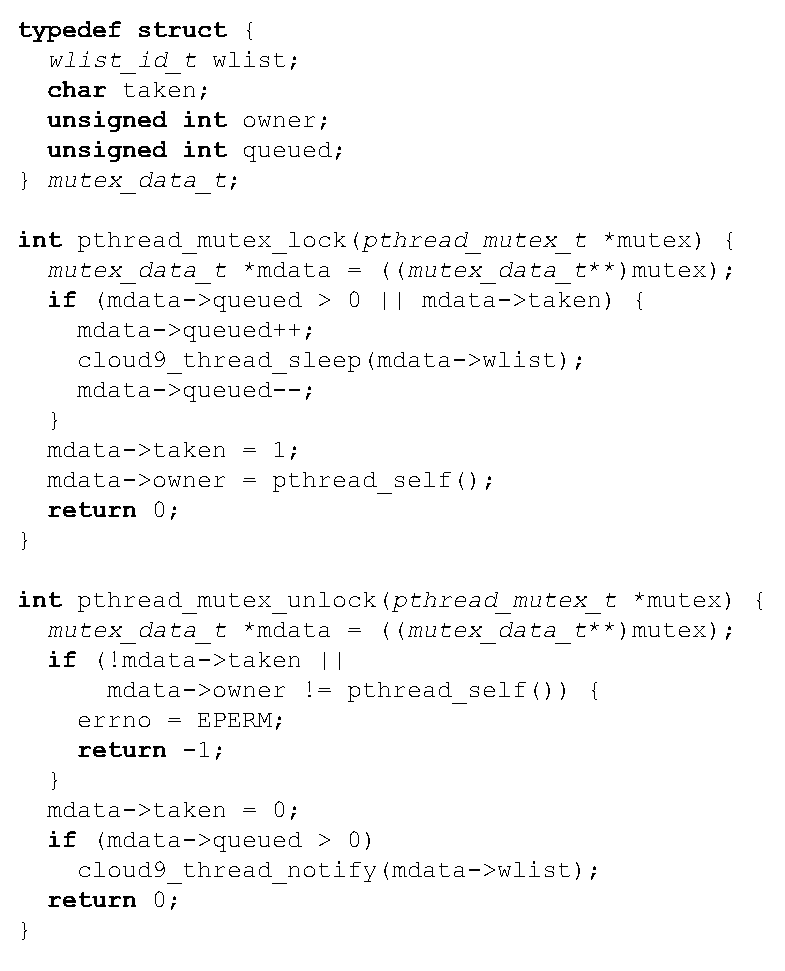
\epsfig{file=figures/cloud9/mutex-model.eps, width=3.2in}
  \caption{Example implementation of pthread mutex operations in \cnine's POSIX environment model.}
  \label{fig:mutexcode}
\end{figure}

\topic{\cnine inherits most of the semantics of the file model from \klee.}  In particular, one can either open a symbolic file (its contents comes from a symbolic block buffer), or a concrete file, in which case a concrete file descriptor is associated with the symbolic one, and all operations on the file are forwarded as external calls on the concrete descriptor. 

\begin{figure}[h!]
  \centering
  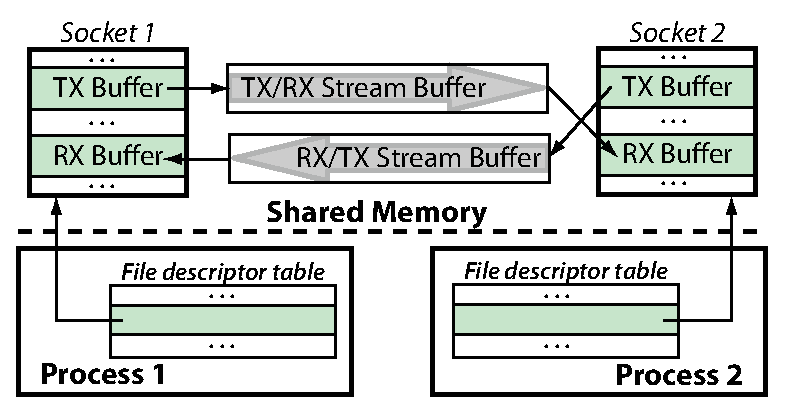
\epsfig{file=figures/cloud9/network-model.eps, width=3.0in}
  \caption{A TCP network connection is modeled in \cnine using TX and RX buffers implemented as stream buffers.}
  \label{fig:networkmodel}
\end{figure}

\topic{In addition to file objects, the \cnine POSIX model adds support for networking and pipes.}  Currently, the TCP and UDP protocols are supported over IP and UNIX network types. Since no actual hardware is involved in the packet transmission, we can collapse the entire networking stack into a simple scheme based on two stream buffers (Fig.~\ref{fig:networkmodel}). The network is modeled as a single-IP network with multiple available ports---this configuration is sufficient to connect multiple processes to each other, in order to simulate and test distributed systems. The model also supports pipes through the use of a single stream buffer, similar to sockets.

\topic{The \cnine POSIX model supports polling through the \codebit{select()} interface.}  All the software we tested can be configured to use \codebit{select()}, so it was not necessary to implement other polling mechanisms.  The \codebit{select()} model relies on the event notification support offered by the stream buffers that are used in the implementation of blocking I/O objects (currently sockets and pipes).

\topic{The constraint solver used in \cnine operates on bit vectors; as a result, symbolic formulas refer to contiguous areas of memory.}  In order to reduce the constraint solving overhead, we aim to reduce the amount of intermixing of concrete and symbolic data in the same memory region.  Thus, \cnine's POSIX model segregates concrete from symbolic data by using static arrays for concrete data and linked lists (or other specialized structures) for symbolic data.  We allocate into separate buffers potentially-symbolic data passed by the tested program through the POSIX interface.

\topic{In order to enable testing the systems presented in the evaluation section (Section~\ref{ch:evaluation}), we had to add support for various other components: IPC routines, \codebit{mmap()} calls, time-related functions, etc.}  Even though laborious, this was mostly an engineering exercise, so we do not discuss it further.


%%%%%%%%%%%%%%%%%%%%%%%%%%%%%%%%%%%%%%%%%%%%%%%%%%%%%%%%%%%%%%%%%%%%%%%%%%%%%%%%

\section{Symbolic Test Suites}

Software products and systems typically have large ``hand-made'' test suites; writing and maintaining these suites requires substantial human effort.  \cnine aims to reduce this burden while improving the quality of testing, by offering an easy way to write ``symbolic test suites.'' First, a symbolic test case encompasses many similar concrete test cases into a single symbolic one---each symbolic test a developer writes is equivalent to many concrete ones.  Second, a symbolic test case explores conditions that are hard to produce reliably in a concrete test case, such as the occurrence of faults, concurrency side effects, or network packet reordering, dropping and delay.  Furthermore, symbolic test suites can easily cover unknown corner cases, as well as new, untested functionality.  In this section, we present the API for symbolic tests and illustrate it with a use case.

\subsection{Testing Platform API}

The \cnine symbolic testing API (Tables~\ref{table:globalapi} and~\ref{table:ioctlapi}) allows tests to programmatically control events in the environment of the program under test.  A test suite needs to simply include a \codebit{cloud9.h} header file and make the requisite calls.

\begin{table}[!t]
\addtolength{\tabcolsep}{-2.5pt}
{
\small
\centering
\begin{tabular}{|l|p{50mm}|}
\hline
\textbf{~~~~~Function Name} & \textbf{~~~~~~~~~~~~~~~~~~Description} \\
\hline
\cninesuffix\_make\_symbolic & Mark memory regions as symbolic \\
\hline
\cninesuffix\_fi\_enable & \multirow{2}{4cm}{Enable/disable the injection of faults} \\
\cninesuffix\_fi\_disable & \\
\hline
\cninesuffix\_set\_max\_heap & Set heap size for symbolic \codebit{malloc} \\
\hline
\cninesuffix\_set\_scheduler & Set scheduler policy (e.g., round-robin)\\
\hline
\end{tabular}
\vspace{-4pt}
\caption{\cnine API for setting global behavior parameters.}
\label{table:globalapi}
}
\end{table}

\begin{table}[!t]
\addtolength{\tabcolsep}{-2.5pt}
{
\small
\centering
\begin{tabular}{|l|p{4.8cm}|}
\hline
\textbf{~~Extended Ioctl Code} & \textbf{~~~~~~~~~~~~~~~~Description} \\
\hline
SIO\_SYMBOLIC & Turns this file or socket into a source of symbolic input \\
\hline
SIO\_PKT\_FRAGMENT & Enables packet fragmentation on this socket (must be a stream socket) \\
\hline
SIO\_FAULT\_INJ & Enables fault injection for operations on this descriptor \\
\hline
\end{tabular}
\vspace{-4pt}
\caption{\cnine extended \codebit{ioctl} codes to control environmental events on a per-file-descriptor basis.}
\label{table:ioctlapi}
}
\end{table}

\paragraph{Symbolic Data and Streams} The generality of a test case can be expanded by introducing bytes of symbolic data. This is done by calling \codebit{\cninesuffix\_make\_symbolic}, a wrapper around \codebit{klee\_\allowbreak{}make\_\allowbreak{}symbolic}, with an argument that points to a memory region. \codebit{klee\_make\_symbolic} is a primitive provided by \klee to mark data symbolic.  In addition to wrapping this call, we added several new primitives to the testing API (Table~\ref{table:globalapi}). In \cnine, symbolic data can be written/read to/from files, can be sent/received over the network, and can be passed via pipes. Furthermore, the \codebit{SIO\_SYMBOLIC} \codebit{ioctl} code (Table~\ref{table:ioctlapi}) turns on/off the reception of symbolic bytes from individual files or sockets.

\paragraph{Network Conditions} Delay, reordering, or dropping of packets causes a network data stream to be fragmented.  Fragmentation can be turned on or off at the socket level using one of the \cnine \codebit{ioctl} extensions.  Section~\ref{sec:eval:lighttpd} presents a case where symbolic fragmentation enabled \cnine to prove that a bug fix for the lighttpd web server was incomplete. 

\paragraph{Fault Injection} Calls in a POSIX system can return an error code when they fail. Most programs can tolerate such failed calls, but even high-quality production software misses some~\cite{lfi}. Such error return codes are simulated by \cnine whenever fault injection is turned on. 

\paragraph{Symbolic Scheduler} \cnine provides multiple scheduling policies that can be controlled for purposes of testing on a per-code-region basis.  Currently, \cnine supports a round-robin scheduler and two schedulers specialized for bug finding: a variant of the iterative context bounding scheduling algorithm~\cite{chess} and an exhaustive exploration of all possible scheduling decisions.  


\subsection{Use Case}

Consider a scenario in which we want to test the support for a new \codebit{X-NewExtension} HTTP header, just added to a web server. We show how to write tests for this new feature.

A symbolic test suite typically starts off as an augmentation of an existing test suite; in our scenario, we reuse the existing boilerplate setup code and write a symbolic test case that marks the extension header symbolic. Whenever the code that processes the header data is executed, \cnine forks at all the branches that depend on the header content. Similarly, the request payload can be marked symbolic to test the payload-processing part of the system:

\begin{verbatim}
   char hData[10];
   cloud9_make_symbolic(hData);
   strcat(req, "X-NewExtension: ");
   strcat(req, hData);
\end{verbatim}

The web server may receive HTTP requests fragmented in a number of chunks, returned by individual invocations of the \codebit{read()} system call---the web server should run correctly regardless of the fragmentation pattern.  To test different fragmentation patterns with \cnine, one simply enables symbolic packet fragmentation on the client socket:
\begin{verbatim}
   ioctl(ssock, SIO_PKT_FRAGMENT, RD);
\end{verbatim}

To test how the web server handles failures in the environment, we can ask \cnine to selectively inject faults when the server reads or sends data on a socket by placing in the symbolic test suite calls of the form:
\begin{verbatim}
   ioctl(ssock, SIO_FAULT_INJ, RD | WR);
\end{verbatim}
\cnine can also enable/disable fault injection globally for all file descriptors within a certain region of the code using calls to \codebit{\cninesuffix\_fi\_\allowbreak{}enable} and \codebit{\cninesuffix\_fi\_\allowbreak{}disable}. For simulating low-memory conditions, \cnine provides a \codebit{\cninesuffix\_set\_\allowbreak{}max\_heap} primitive, which can be used to test the web server with different maximum heap sizes.

%%% Local Variables: 
%%% mode: latex
%%% eval: (visual-line-mode)
%%% fill-column: 1000000
%%% TeX-master: "main"
%%% End:
